\section{Motor control}
As mentioned in the introduction, the target rotating speed is 30 rps.
In order to ensure this, a PID controller is implemented to keep the speed constant.
Since the motor chosen for the project does not have encoders build in, so in order to get some feedback for the controller, 3 hall sensors are implemented.
A ramp up function is also implemented.

\subsection{Controller}

To ensure a smooth picture the pcb should rotate at a constant speed.
This is done using a P controller, with a gain that is not too big since overshoot is not desirable.

\subsection{Encoders} \label{sec:encoders}
%trim = left botm right top
\begin{wrapfigure}{r}{0.7\textwidth}
 \caption{Schematic of the board that is mounted under the spinning board}
 \label{fig:botm_schematic}
 \centering
 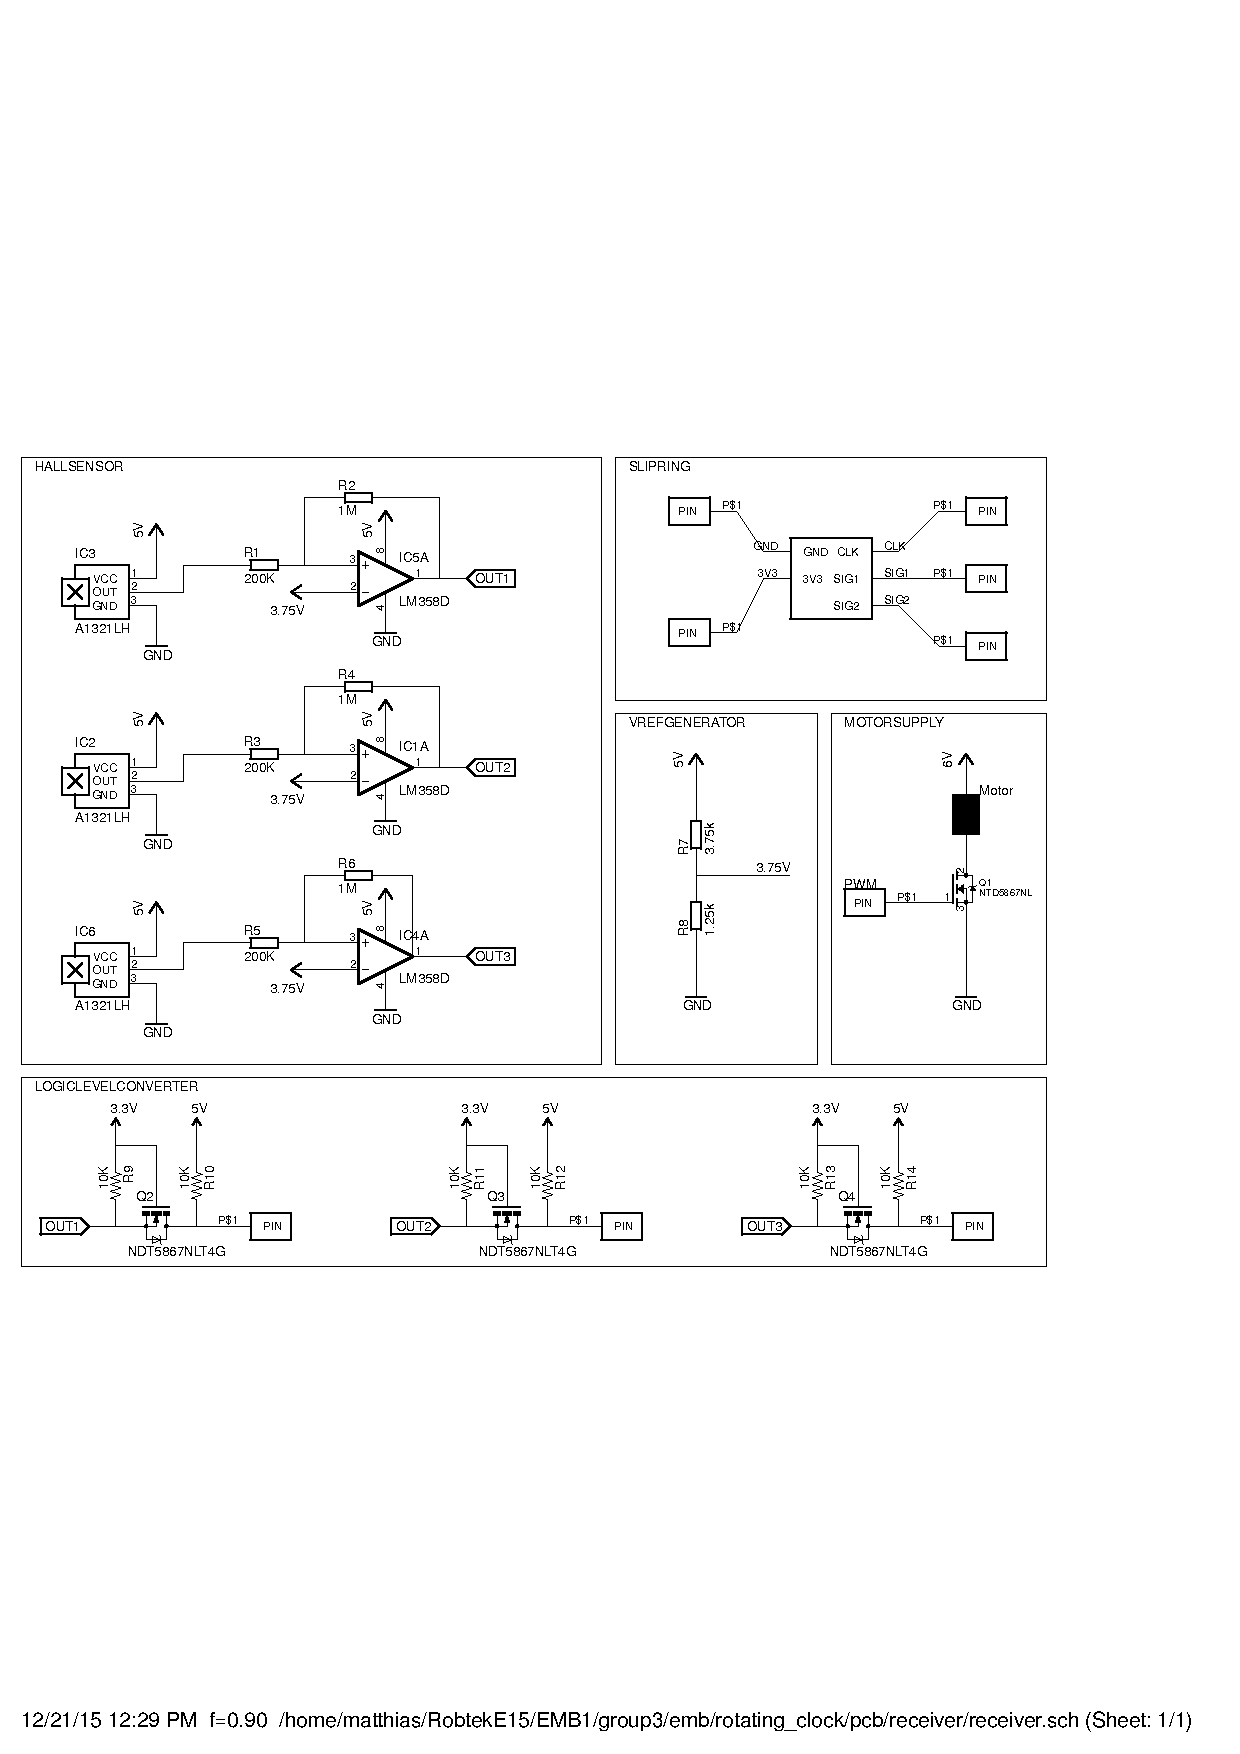
\includegraphics[scale = 0.5,trim = 0 14.5cm 8cm 0,clip = true]{img/bottompcb_schematic}
\end{wrapfigure}

In order to calculate the current speed of the pcb, 3 hall sensor are mounted on the board located under the rotating pcb, and a magnet is mounted on the rotating pcb.
The hall sensors have been placed with $120^{\circ}$ between them.

In order to get a binary from the analog hall sensor, a schmitt trigger is added on the output of the hall sensor.
The choice of using a schmitt trigger instead of a standard comparator is to reduce sensor noise when the magnet is moving over the sensor.

The speed is can be calculated by counting up a counter between getting logic high from one of the hall sensors to  logic high on one of the others, using equations  \ref{eq:calc_time} and \ref{eq:calc_speed}.

\begin{equation} \label{eq:calc_time}
 t = \frac{20\cdot \text{counter}}{1\cdot 10^9}
\end{equation}

\begin{equation} \label{eq:calc_speed}
 \text{speed} = \frac{1}{3\cdot t}
\end{equation}

\subsubsection{Bottom board}
The schematic for the pcb can be seen in figure \ref{fig:botm_schematic}.
On the board is as mentioned the three hall sensors with a schmitt trigger for each, as well as the bottom of the slip ring. The slip ring setup and design can be seen in section \ref{sec:ring_connector}. 


\subsection{Ramp up}

The ramp up function is implemented to get a faster speed up time.
If this is not implemented, either an aggressive controller has to be implemented for the entire system, which is not desirable, or the time to reach the desired speed will become very long.

Instead of this, another controller is implemented, which is basically just an integrator.
When the integrator reaches a specified speed, the regular controller takes over. 